\subsection{STT}
\label{subsec:stt}

\paragraph{STT}
\textbf{S}ingle \textbf{T}arget \textbf{T}rack
\begin{itemize}
    \item \textbf{FCR continually scans one target}
    \begin{itemize}
        \item high update frequency \& precision for weapon guidance
        \item \underline{target RWR will detect STT lock}
    \end{itemize}
    \item \textbf{FCR search ceases during STT lock}
    \item \textbf{Entered by}
    \begin{itemize}
        \item locking bugged target from \textbf{TWS/RWS} with \textbf{TMS Forward}
        \item placing target in search volume of \textbf{ACM} (lock occurs automatically)
    \end{itemize}
    \item \textbf{Exited with TMS Aft} --- returns to search mode
\end{itemize}

\paragraph{Display}
\begin{itemize}
    \item \textbf{Target state} shown at top of FCR page
    \begin{itemize}
        \item aspect angle 
        \item ground track 
        \item airspeed 
        \item closure rate
    \end{itemize}
\end{itemize}

\paragraph{NCTR}
\textbf{N}on-\textbf{C}ooperative \textbf{T}arget \textbf{R}ecognition
\begin{itemize}
    \item \textbf{FCR attempts to identify locked target}
    \begin{itemize}
        \item measures turbine parameters to produce \underline{likely} contact aircraft type
        \item NCTR is only available in STT
    \end{itemize}
    \item \textbf{NCTR imposes additional requirements}
    \begin{itemize}
        \item target must be within 20-25nm
        \item radar must ``see'' compressor/turbine blades
    \end{itemize}
    \item \textbf{Activated with IFF interrogation (TMS Left long)}
    \item \textbf{Hostile NCTR identification counts towards ROE matrix} (combined with IFF return)
\end{itemize}

\begin{figure}[htbp]
    \centering
    \begin{tikzpicture}[auto, node distance=10mm, x=1mm, y=1mm, very thick, line cap=round,
        >={Latex[round]}
        ]
        
        \node[] (fig) at (0,0) {
            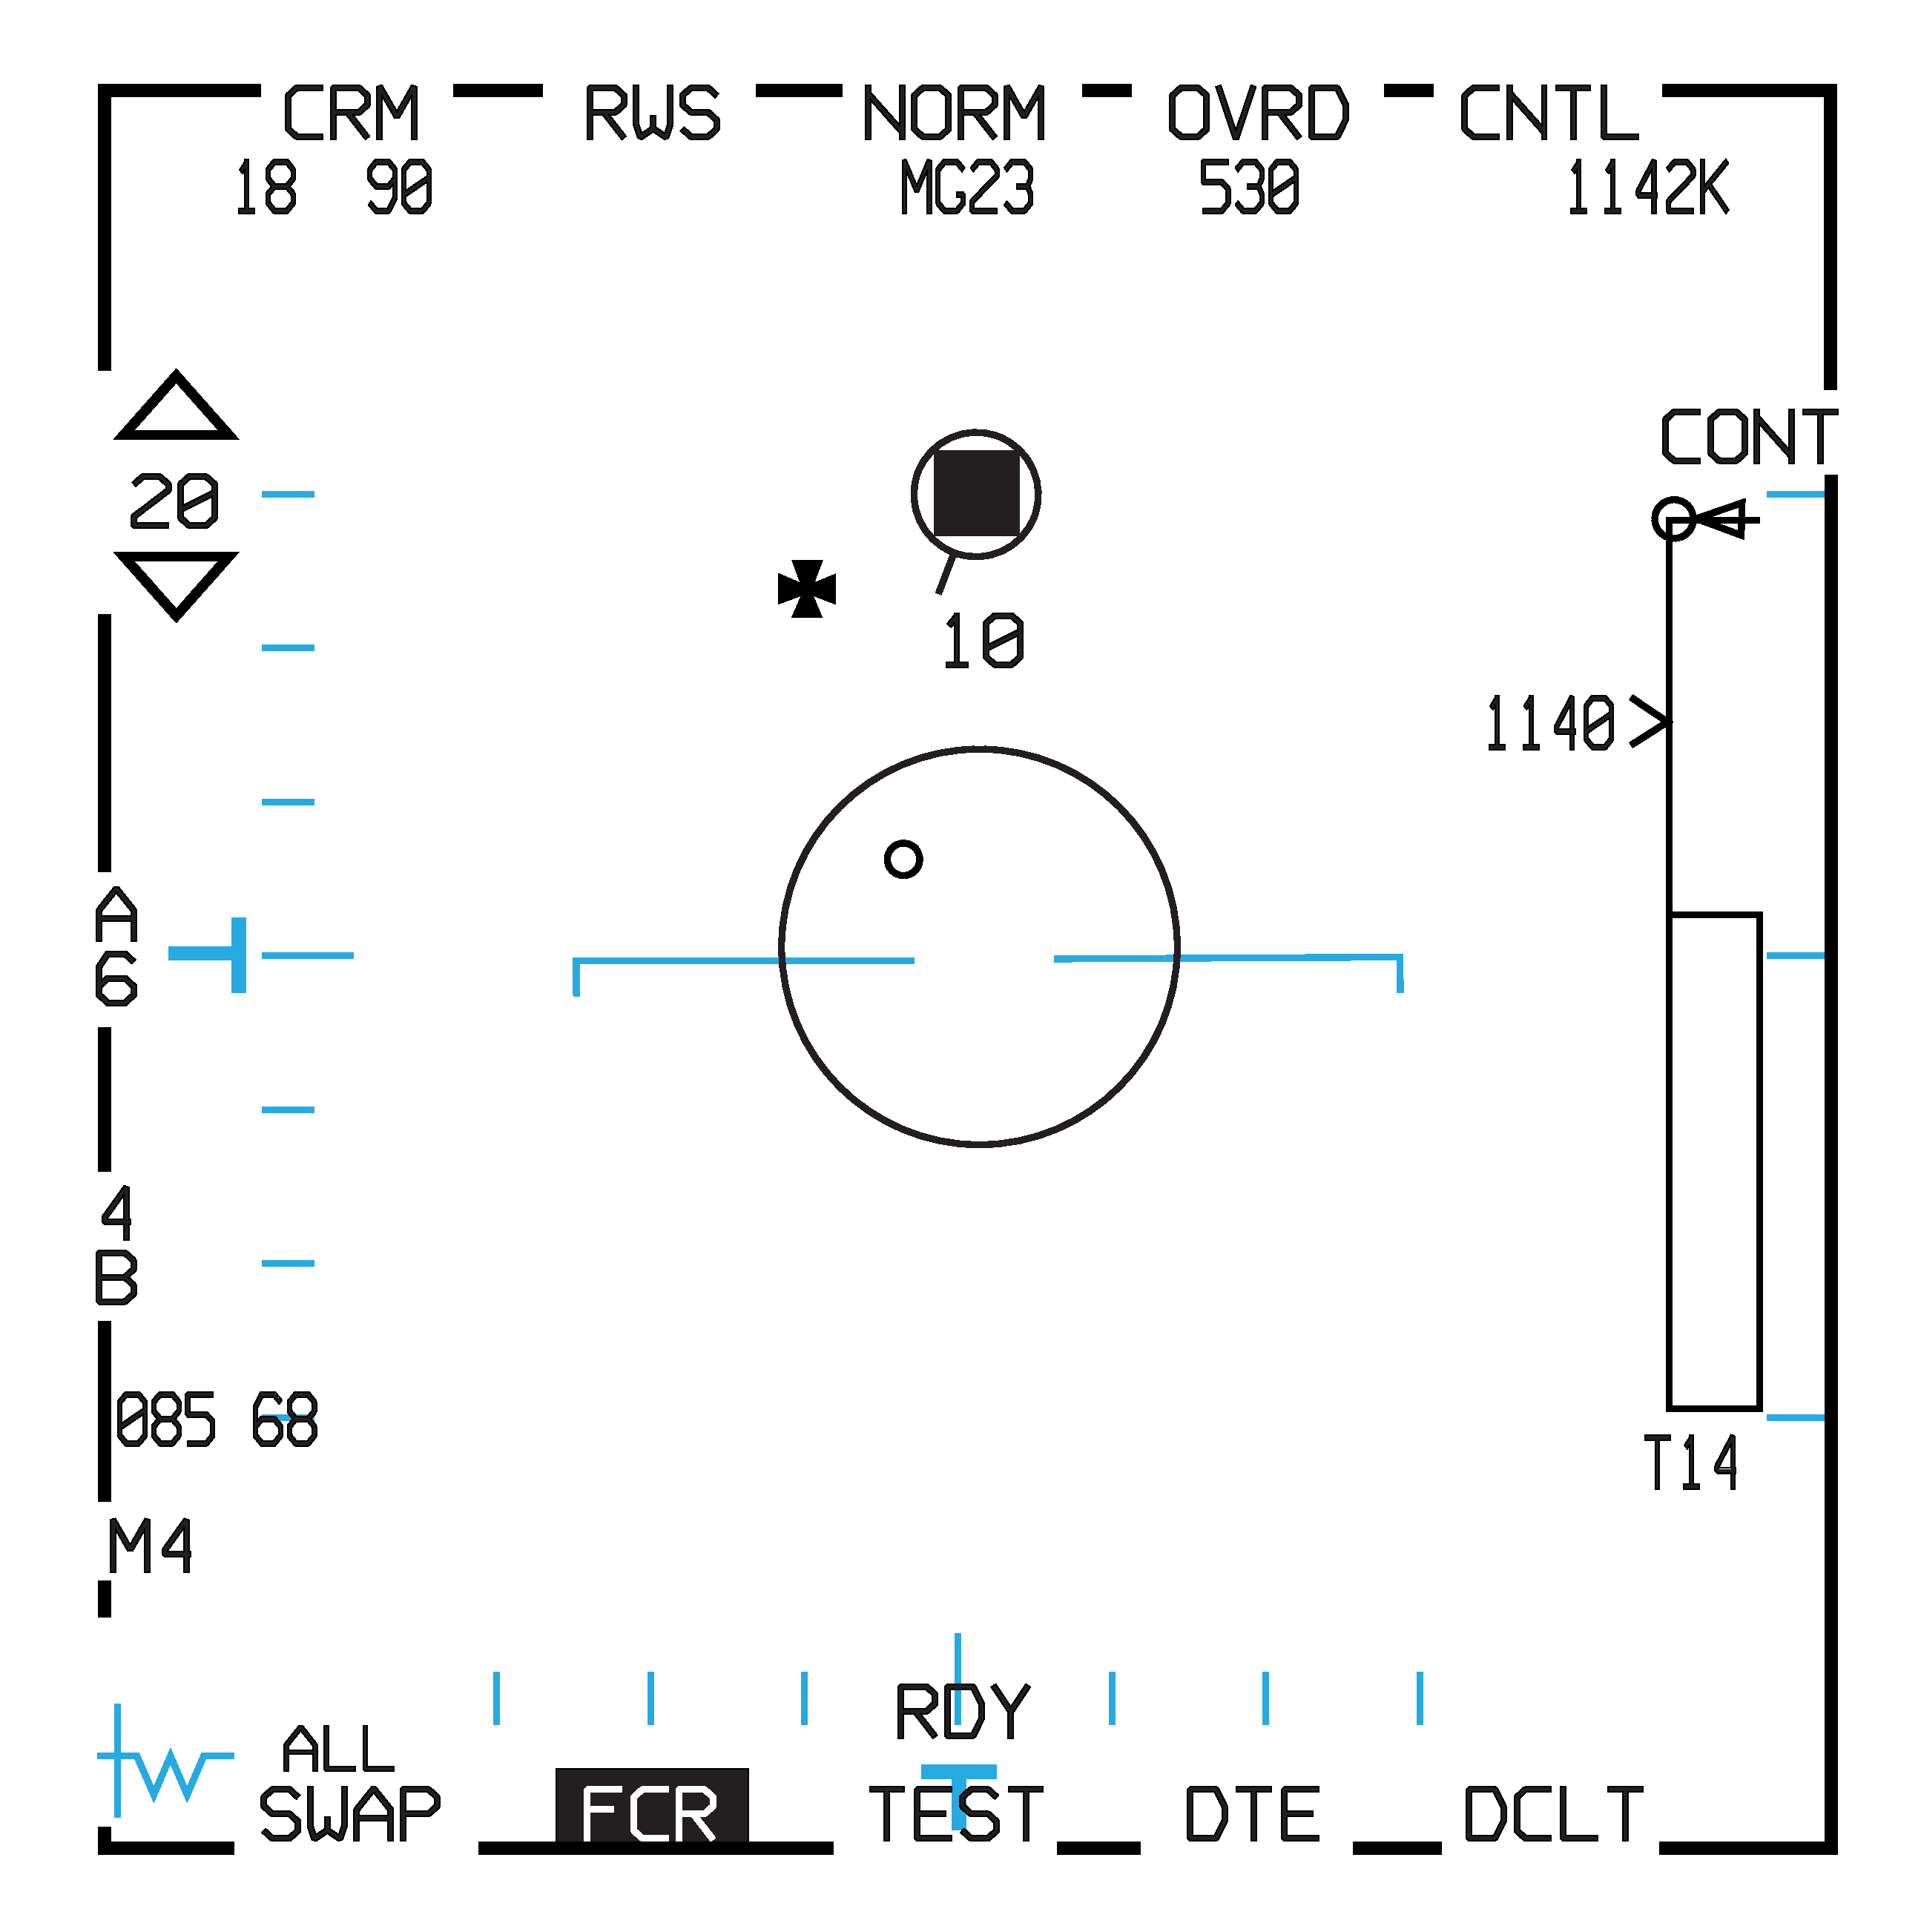
\includegraphics[
                height=75mm,
            ]{mfd/fcr_aa/stt_nctr.pdf}
        };

        % Annotations
        \node[lannot] (asp) at ($(fig.west)+(0mm,30.25mm)$) {Aspect};
        \draw[annotptr] (asp.east) -- ++(9mm, 0mm);

        \node[lannot] (trk) at ($(fig.west)+(0mm,24mm)$) {Track};
        \draw[annotptr] (trk.east) -- ++(12mm, 0mm) -- ++(4mm, 4mm);

        \node[lannot] (cross) at ($(fig.west)+(0mm,9mm)$) {Steering \\ cross};
        \draw[annotptr] (cross.east) -- ++(27mm, 0mm) -- ++(4mm, 4mm);

        \node[lannot] (asec) at ($(fig.west)+(0mm,-8mm)$) {ASC / ASEC \\ {\footnotesize see \cref{fig:aa_weap:aim120:asc_asec}}};
        \draw[annotptr] (asec.east) -- ++(28mm, 0mm) -- ++(4mm, 4mm);

        \node[rannot] (clos) at ($(fig.east)+(0mm,30.25mm)$) {Closure};
        \draw[annotptr] (clos.west) -- ++(-8mm, 0mm);

        \node[rannot] (as) at ($(fig.east)+(0mm,24mm)$) {Airspeed};
        \draw[annotptr] (as.west) -- ++(-22mm, 0mm) -- ++(-4mm, 4mm);

        \node[rannot] (bug) at ($(fig.east)+(0mm,12mm)$) {STT \\ Target};
        \draw[annotptr] (bug.west) -- ++(-32mm, 0mm) -- ++(-4mm, 4mm);

        \node[rannot] (dlz) at ($(fig.east)+(0mm,2mm)$) {DLZ \\ {\footnotesize see \cref{fig:aa_weap:aim120:dlz}}};
        \draw[annotptr] (dlz.west) -- ++(-7mm, 0mm);

        \node[annot, anchor=south, align=center] (nctr) at ($(fig.north)+(-7mm,0mm)$) {NCTR ID};
        \draw[annotptr] (nctr.south) -- ++(0mm, -8.5mm) -- ++(4mm, 0mm);
    \end{tikzpicture}
    \caption{RWS FCR page with STT lock and NCTR ID.}
\end{figure}